\documentclass{article}
\usepackage{enumerate}
\usepackage{amsmath}
\usepackage{amssymb}
\usepackage{graphicx}
\usepackage{subfigure}
\usepackage{geometry}
\usepackage{color}
\usepackage{bm}
\usepackage{indentfirst}
\usepackage{multirow}

\begin{document}

\vspace*{0.25cm}

\hrulefill

\thispagestyle{empty}

\begin{center}
\begin{large}
\sc{UM--SJTU Joint Institute \vspace{0.3em} \\ Circuits Laboratory \\(VE215)}
\end{large}

\hrulefill

\vspace*{5cm}
\begin{Large}
\sc{{Laboratory Report}}
\end{Large}

\vspace{2em}

\begin{large}
\sc{{Exercise 1
\vspace{0.5em}

DC Lab
}}
\end{large}
\end{center}


\vfill

\begin{table}[h!]
\flushleft
\begin{tabular}{lll}
Name: Yihao Liu \hspace*{2em}&
ID: 515370910207\hspace*{2em}\\
& Section: 3\\


\\

Date: 13 Oct 2016 

\end{tabular}
\end{table}

\hfill
\begin{tiny}
[rev. 1.0]
\end{tiny}
\newpage

\section{Introduction}
\subsection{Goals for the Lab}
\begin{enumerate}[i.]
\item
Learn how to use UT60A multimeter for measurements of voltage, current, and resistance.
\item
Learn to build circuits on a solderless prototype board.
\item
Verify the basic circuit laws KCL, KVL, and Ohm’s laws from measurements of currents and voltages.
\item
Measure the current-voltage characteristics of a 50$\Omega$ resistor. From the results of measurements, draw the conclusion on whether they obey Ohm’s law.
\item
Build an LED circuit on a protoboard and learn about non-ohmic circuit components, which do not obey Ohm’s law.
\end{enumerate}

\subsection{Experimental Instruments}
\subsubsection{Multimeter}
A multimeter is able to work as a voltmeter to measure voltages, as an ammeter to measure currents, or as an ohmmeter to measure resistances.
Every multimeter has two terminals for the two cables that ensure electrical connections to the two nodes. The black cable should be connected to ground, the ground port is labeled COM on the multimeter. The red cable should be connected to HzV$\Omega$ port for voltage or resistance measurements, 10A MAX port for current measurements, or $\mu$AmA port for small current measurements.
\paragraph{Voltage Measurements}
The voltmeter has its own internal resistance, which is usually very high. For an ideal voltmeter the input resistance is infinitely large. In real instruments the internal resistance usually exceeds 1M$\Omega$. When we measure $V_{AB}$ the voltmeter’s internal resistance is connected in parallel with all circuit elements between these two terminals. Note that you do not have to change anything in your circuit to measure voltage: just connect the multimeter to the nodes of interest.
\paragraph{Current Measurements}
To measure the current that flows through a branch of your circuit we should make this current flow through the multimeter. Note that in order to measure the current we have to interrupt the circuit.
\paragraph{Resistance Measurements}
To measure the resistance, we simply connect it to the two terminals of the multimeter, and read the resistance from the display. Remember: you must disconnect the resistor from your circuit before measuring the resistance! Otherwise, you will not obtain the correct reading of resistance.
\subsubsection{DC source}
\paragraph{LPS 305 Power Supply}
\begin{enumerate}[1.]
\item
When you press the +Vset, or -Vset, the output selected (+output or –output) and the present setting for that function will be displayed. You can change setting using the numeric entry keys. Pressing the number keys will cause the present numeric setting to become blank and be replaced with the new numbers on the display. Pressing the ENTER key will enter the values displayed.
\item
The selected output channel can be turned on and off from the front panel. The output on/off key toggles both the +output and –output on and off simultaneously.
\item
Remember to turn off the output when no measurements are being undertaken.
\end{enumerate}
\paragraph{Agilent E3631A DC Power Supply}
To set up the power supply for constant voltage (CV) operation, proceed as follows. 
\begin{enumerate}[1.]
\item
Connect a load to the desired output terminals with power-off.
\item
Press to turn on the power supply. The power supply will go into the power-on / reset state; all outputs are disabled (the OFF annunciator turns on); the display is selected for the +6V supply (the +6V annunciator turns on); and the knob is selected for voltage control.
\item
Adjust the knob for the desired output voltage. Set the knob for voltage control. The second digit of the voltmeter will be blinking. Adjust the knob to the desired output voltage.
\end{enumerate}

\subsubsection{Protoboards}
In this lab and all the future labs, you will connect resistors, LEDs and other components to each other on a circuit board. Circuits boards are also called “protoboards”, because they are used for prototyping the circuits. Another name is “breadboard”, because in old times circuits were indeed built on wooden breadboards. The main idea is to build the citcuit without soldering every connection thus the long generic name is solderless prototyping boards.

A prototyping board used in the lab consists of several plastic blocks. These plastic blocks are mounted on a metal plate along with terminal (blind) posts.

Each plastic block has many holes, into which you insert wires, plug in resistors, op amps, and other circuit components. Inside the plastic block, themetal clips snugly hold your wires, resistors, etc., and ensure electric connections between circuit components.

\subsubsection{Semiconductor diodes}
The simplest semiconductor device is a diode. Its circuit symbol looks like an arrow because the diode allows the current flow only in the direction of that arrow. If $V_A>V_B$ (which is called direct bias) the conductor will conduct. If $V_A<V_B$ (which is called reverse bias) the conductor will not conduct. Thus a diode is not an Ohmic resistor.

Moreover, even under direct bias the resistance of a diode does not remain constant. At small values of the voltage difference $V_A-V_B$ the current through the diode is very small, because its resistance is large. The diode’s resistance abruptly changes as soon as the direct bias voltage across the diode reaches the threshold value, which is called the turn-on voltage and equals about 0.5 to 0.7V for many diodes. Above this voltage the current through the diode rapidly increases and becomes practically independent of the voltage. The diode resistance becomes so small that in real circuits the diodes have to be protected from high currents that may damage them. A load resistor (50$\Omega$ in this lab) connected in series with the diode ensures the simplest protection.
Light-emitting diodes emit light (visible or infrared) when the direct current becomes large enough. The LED, which you will use in this lab, has the turn-on voltage of about 1.6V. 

\subsection{Procedures}
\subsubsection{Voltage, Current \& Resistance Measurement}
\begin{enumerate}[a)]
\item
Use the multimeter to measure the resistance $R_1$ labeled 100$\Omega$ directly and record the result.
\item
Connect the resistance $R_1$ = 100$\Omega$ with the power supply and set the voltage 3V.
\item
Use the multimeter to measure the Voltage (m) across the resistor and compare it with the Voltage (s) shown on the power supply.
\item
Use the multimeter to measure the Current (m) through the resistor and compare it with the Current (s) shown on the power supply.
\end{enumerate}

\subsubsection{Voltage Division \& Current Division}
\begin{enumerate}[a)]
\item
Before measurement, measure the actual resistances of the two resistors you are using in this section.
\item
Connect the $R_1$ = 100$\Omega$ and $R_2$ = 50$\Omega$ in series and in parallel, respectively.
\item
Use the multimeter to measure the voltage across the $R_1$, $R_2$ and the power supply, and think about the relationship among the three voltages.
\item
Use the multimeter to measure the current through $R_1$, $R_2$ and the power supply, and think about the relationship among the three currents.
\item
Compare the result with what you expect.
\end{enumerate}

\subsection{Ohm’s Law}
\begin{enumerate}[a)]
\item
Measure the resistance of R = 50$\Omega$ and record the result.
\item
Connect the R with the power supply.
\item
Set the voltage outputs and record the corresponding currents.
\item
Sketch the voltage-current characteristic curve of the resistor.
\end{enumerate}

\subsection{Non-ohmic LED}
\begin{enumerate}[a)]
\item
Connect the resistor R = 50$\Omega$ and the LED in series with the power supply.
\item
Change the voltage output and record the corresponding current.
\item
You need to design the proper step of voltages to get the voltage-current characteristic of the non-ohmic device.
\end{enumerate}
\section{Results \& Discussion}
\subsubsection{Voltage, Current \& Resistance Measurement}
\begin{table}[!h]
\begin{center}
\begin{tabular}{|c|c|c|c|c|}
\hline
Resistance[$\Omega$]	&	\multicolumn{3}{|c|}{98.5}\\
\hline
Voltage(m)[V]	&	2.998	&	Voltage(s)[V]	&	3.000\\
\hline
Current(m)[A]	&	0.0302	&	Current(s)[A]	&	0.031\\
\hline
\end{tabular}
\caption{Measurement of voltage, current and Resistance.}
\label{tab-1}
\end{center}
\end{table}
According to the data, we can find that the results form the multimeter have some tiny difference from the theoretical ones.

\subsubsection{Voltage Division \& Current Division}
\begin{table}[!h]
\begin{center}
\begin{tabular}{|c|c|c|c|c|c|}
\hline
\multicolumn{2}{|c|}{Resistance $R_1$[$\Omega$]} & 98.5 &
\multicolumn{2}{|c|}{Resistance $R_2$[$\Omega$]} & 47.1\\
\hline
\multicolumn{2}{|c|}{\multirow{2}{*}{}} & \multicolumn{2}{|c|}{Voltage Division} &
\multicolumn{2}{|c|}{Current Division}\\
\cline{3-6}
\multicolumn{2}{|c|}{} & Current [A] & Voltage [V] & Current [A] & Voltage [V]\\
\hline
\multicolumn{2}{|c|}{Total}	&	0.020	&	2.998	&	0.094	&	2.993\\
\hline
\multicolumn{2}{|c|}{$R_1$}	&	0.020	&	2.038	&	0.0302	&	2.992\\
\hline
\multicolumn{2}{|c|}{$R_2$}	&	0.020	&	0.960	&	0.0631	&	2.990\\
\hline
\end{tabular}
\caption{Voltage division and current division.}
\label{tab-2}
\end{center}
\end{table}
According to the data, we can find that in a series circuit, the current in each resistance is the same, and the voltage is divided by the value of the resistances. In a parallel circuit, the voltage on each resistance is the same, and the current is divided by the reciprocal of the value of the resistances.

\subsection{Ohm’s Law}
\begin{table}[!h]
\begin{center}
\begin{tabular}{|c|c|}
\hline
Resistance[$\Omega$]	&	47.1\\
\hline
Voltage [V]	& Current [A]\\
\hline
0.5	&	0.011\\
1.0	&	0.022\\
1.5	&	0.034\\
2.0	&	0.044\\
3.0	&	0.066\\
4.0	&	0.088\\
5.0	&	0.111\\
\hline
\end{tabular}
\caption{Ohm’s Law.}
\label{tab-3}
\end{center}
\end{table}
\begin{figure}[!h]
	\centering
	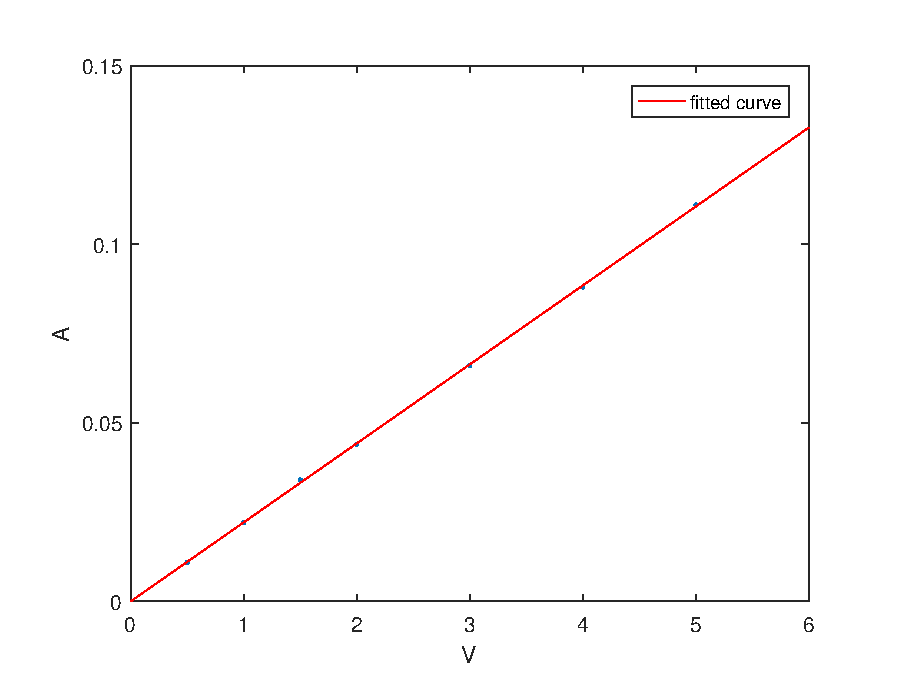
\includegraphics[width=10cm]{lab1_.eps}
	\caption{V-A curve.
	\label{fig-1}}
\end{figure}
$$\frac{1}{k}=\frac{1}{0.0221}=45.25$$
According to the data and the plot, we can verify the Ohm’s Law
$$R=\frac{U}{I}$$

\subsection{Non-ohmic LED}
\begin{table}[!h]
\begin{center}
\begin{tabular}{|c|c|}
\hline
Voltage [V]	& Current [A]\\
\hline
0.998 & 0.000\\
1.674 & 0.003\\
1.713 & 0.007\\
1.741 & 0.010\\
1.812 & 0.022\\
1.884 & 0.035\\
2.038 & 0.066\\
2.252 & 0.107\\
2.506 & 0.171\\
\hline
\end{tabular}
\caption{Semiconductor diodes.}
\label{tab-3}
\end{center}
\end{table}
\begin{figure}[!h]
	\centering
	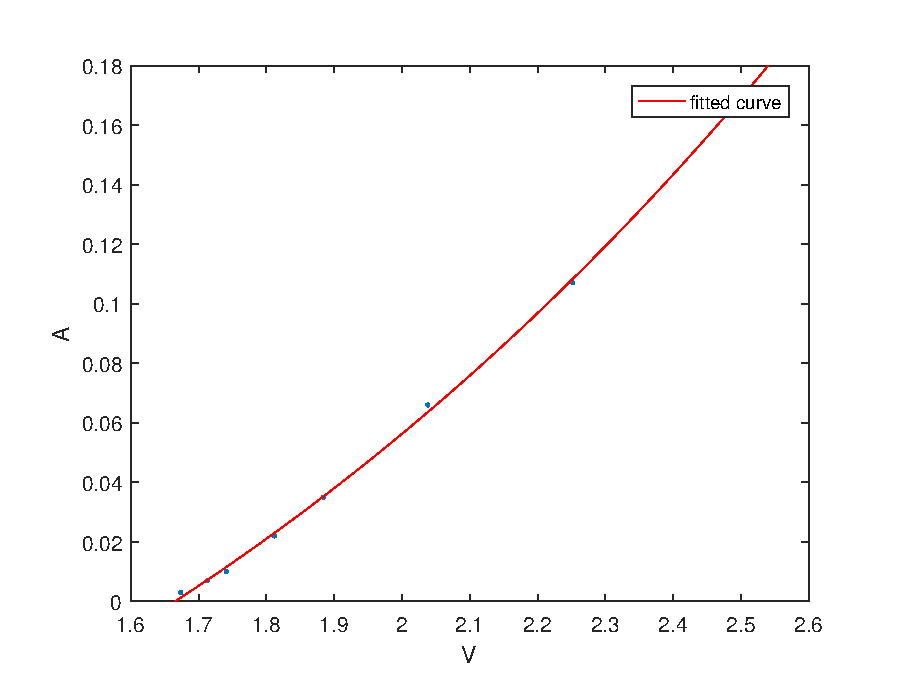
\includegraphics[width=10cm]{lab1.eps}
	\caption{V-A curve.
	\label{fig-1}}
\end{figure}
According to the data, I use MATLAB to plot a V-A curve.


\section{Conclusion}
In the experiment, I learned how to use UT60A multimeter for measurements of voltage, current, and resistance and built circuits on a solderless prototype board. I also verified the basic circuit laws KCL, KVL, and Ohm’s laws from measurements of currents and voltages. I measured the current-voltage characteristics of a 50$\Omega$ resistor. From the results of measurements, draw the conclusion on whether they obey Ohm’s law. I Built an LED circuit on a protoboard and learn about non-ohmic circuit components, which do not obey Ohm’s law.

\section{Reference}
Circuits Make Sense, Alexander Ganago, Department of Electrical Engineering and Computer Science, University of Michigan, Ann Arbor.

\section{Data sheet}





\end{document}

